\documentclass[serif,9pt]{beamer}
\setbeamertemplate{navigation symbols}{}

\usepackage[utf8]{inputenc}
\usepackage[T1]{fontenc}
\usepackage[catalan]{babel}

\usetheme{Warsaw}
\usecolortheme{seahorse}

\beamersetuncovermixins{\opaqueness<1>{25}}{\opaqueness<2->{15}}

\AtBeginSection[]
{
  \begin{frame}<beamer>
    \frametitle{Continguts}
    \tableofcontents[currentsection]
  \end{frame}
}


\begin{document}

\title[Quadriga]{Quadriga: Plataforma de Programació en Sistemes d'Entitats, per al desenvolupament de Videojocs}  
\author{Isaac Serrano}
\institute{Universitat Autònoma de Barcelona}
\date{7 de Juliol del 2011}

\begin{frame}
\titlepage
\end{frame}

\begin{frame}
\frametitle{Continguts}
\tableofcontents
\end{frame}

\section{Introducció}

  \subsection{Motivació}

    \begin{frame}\frametitle{Motivació}
     \begin{itemize}
      \item Augment de la complexitat en la creació de videojocs. \pause
      \item Surt més a compte comprar un motor que crear-lo. \pause
      \item Molts motors disponibles, fins i tot lliures (Ogre, jMonkeyEngine, etc.).\pause
      \item Com crear un joc sobre aquests motors? Mòdul de Lògica.
     \end{itemize}
    \end{frame}

    \begin{frame}\frametitle{Mòdul de Lògica}
      \begin{itemize}
        \item Ha de permetre crear els objectes del joc (arbres, vegetació, monstres, nivells, portes, herois, objectes d'inventari, triggers, seqüències de càmera...) i el seu comportament (renderitzar, cerca de camins, animar, fer decisions d'IA...).\pause
        \item Ha de crear/destruir els objectes en el joc i coordinar els missatges entre ells.\pause
        \item Ha de mantenir una BBDD dels objectes actius, i crear-se a partir d'una altra BBDD estàtica (que defineix el joc).\pause
        \item Esquemàticament, {\bf tots} els jocs tenen això d'una manera o altra.
      \end{itemize}
    \end{frame}

    \begin{frame}\frametitle{Esquema original}
      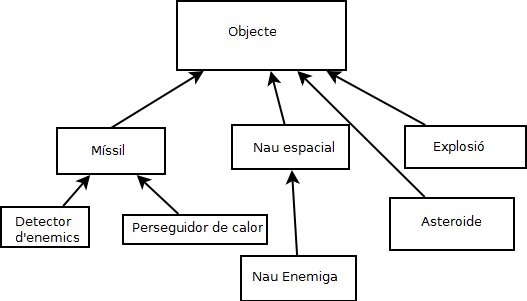
\includegraphics[width=1.00\textwidth]{./img/DiagramaObjectes1.png}
    \end{frame}

    \begin{frame}\frametitle{Refacció}
      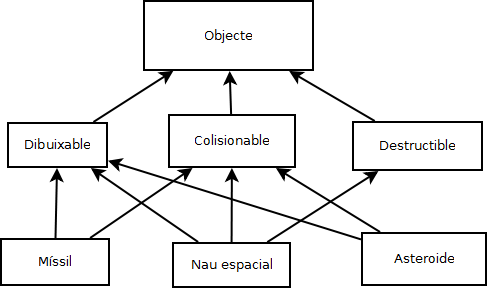
\includegraphics[width=1.00\textwidth]{./img/DiagramaObjectes2.png}
    \end{frame}

    \begin{frame}\frametitle{Refacció en Components}
      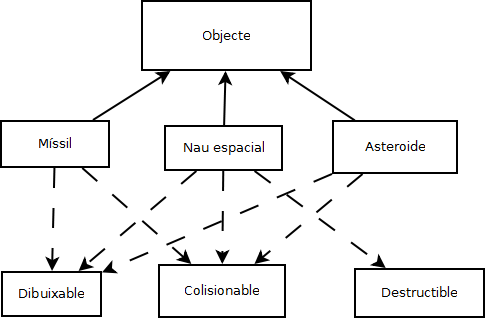
\includegraphics[width=1.00\textwidth]{./img/DiagramaObjectes3.png}
    \end{frame}
    
  \subsection{Objectius}

    \begin{frame}\frametitle{Objectius}
      \begin{itemize}
        \item Crear un mòdul de Lògica. \pause
        \item Dirigida per dades, poder prescindir dels enginyers. \pause
        \item Open Source. \pause
        \item Multi-plataforma. \pause
        \item Paral·lelitzable.
      \end{itemize}
    \end{frame}

\section{Desenvolupament}

  \subsection{Disseny}

    \begin{frame}\frametitle{Disseny}
      \begin{itemize}
        \item Crear un llenguatge de programació, Quadriga. \pause\medskip
        \begin{itemize}
          \item Components.
          \item Sistemes.
          \item Events.
          \item Prototips.
          \item Thread, Main.
        \end{itemize}\pause
        \item Crear un entorn d'execució: dirigir events, mantenir la BBDD.
      \end{itemize}
    \end{frame}
  
    \begin{frame}\frametitle{Desenvolupament}
      \includegraphics[width=1.00\textwidth]{./img/EsquemaExecució.png}
    \end{frame}

  \subsection{Compilador}
    \begin{frame}\frametitle{Compilador}
      \begin{itemize}
        \item Desenvolupat amb JavaCC a partir de la gramàtica de Java 1.5.\pause
        \item El compilador crea un arbre sintàctic i aquest s'executa.\pause
        \item El compilador també crea la base de dades, específica per al joc.
      \end{itemize}
    \end{frame}
    
  \subsection{Entorn d'execució}
    
    \begin{frame}\frametitle{Entorn d'execució}
      \begin{itemize}
        \item Treballa directament a la JVM. Permet usar classes escrites Java sense dificultats. \pause
        \item Conté una base de dades. Usa HSQLDB i permet guardar tipus primitius i classes {\em Seriallizable}. \pause
        \item S'encarrega de la creació i destrucció d'elements, de la modificació de dades i de la comunicació amb events.
      \end{itemize}
    \end{frame}

    
    \begin{frame}\frametitle{Base de Dades}
      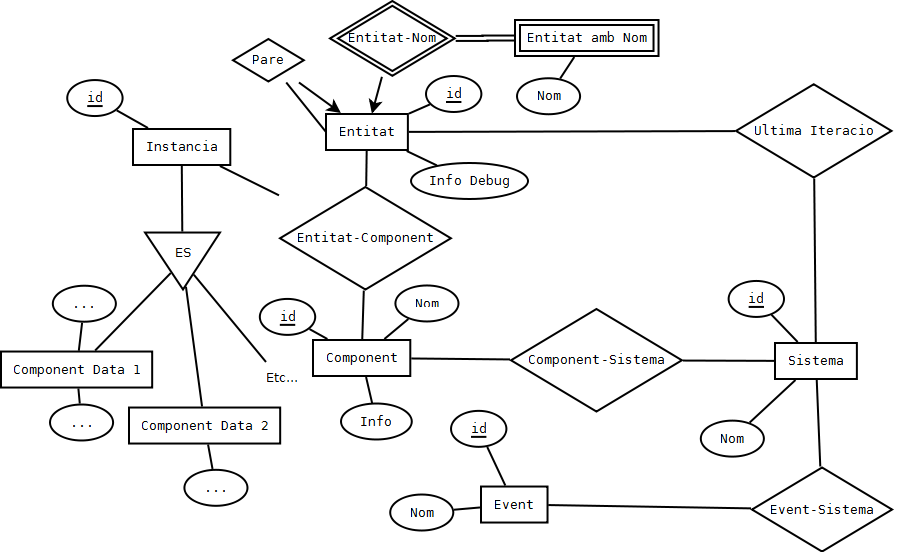
\includegraphics[width=1.00\textwidth]{./img/EntitatRelacio2.png}
    \end{frame}

\section{Resultats}

  %Tetris
  \begin{frame}\frametitle{Resultats}
    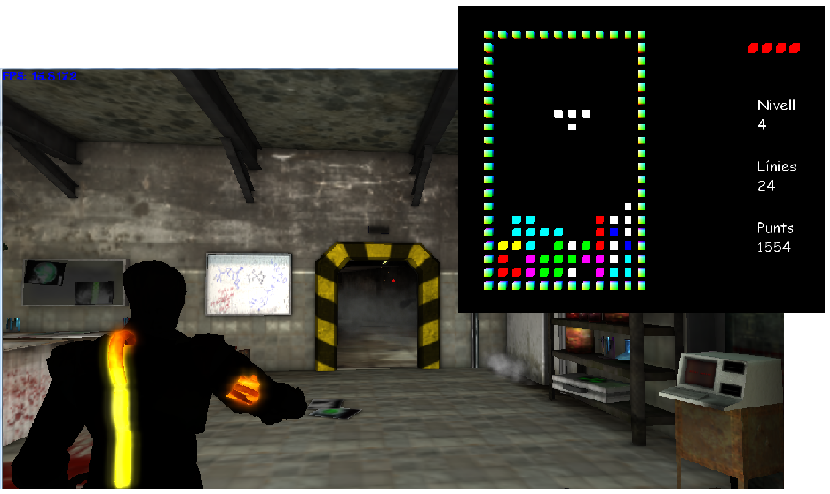
\includegraphics[width=1.00\textwidth]{./img/Screens.png}
  \end{frame}

\section{Conclusions i Millores}

  \begin{frame}\frametitle{Conclusions}
    \begin{itemize}
      \item S'ha dissenyat un llenguatge de programació que segueix el paradigma dels {\em Sistemes d'Entitats} i s'ha anomenat Quadriga.
      \item S'ha dissenyat i implementat un {\bf compilador} per aquest llenguatge.
      \item S'ha implementat un {\bf entorn d'execució} que proporcioni al programa tots els elements necessaris per al seu correcte funcionament en qualsevol plataforma suportada per Java.
      \item S'ha creat una base de dades especificada dinàmicament (resultat de la compilació) que suporta qualsevol tipus de joc sobre un format estandaritzat.
      \item S'ha creat un subratllador de sintaxi per facilitar la seva programació.
      \item S'ha implementat un joc d'exemple basat en el clàssic {\bf Tetris}.
      \item S'ha desenvolupat una petita llibreria bàsica per a renderitzar textos i algunes formes geomètriques simples: cubs i esferes.
      \item S'ha dissenyat un model de llibreria tal que sigui fàcil de transportar a altres plataformes (fins i tot plataformes mòbils) emprant les últimes tècniques de renderitzat (mitjançant els {\em Shaders} d'OpenGL 2.0).
    \end{itemize}
  \end{frame}
  
  \begin{frame}\frametitle{Millores}
    \begin{itemize}
      \item Fer que el compilador generi bytecode per executar directament a la màquina virtual de Java, millorant el rendiment dels programes desenvolupats a Quadriga.
      \item Crear una implementació específica del model de dades, sense usar una base de dades SQL. Així el rendiment milloraria considerablement.
      \item Ampliar la llibreria estàndard per incloure la següent funcionalitat:
      \begin{itemize}
        \item Renderitzar formes geomètriques arbitràries (actualment només se suporten cubs, esferes i textos).
        \item Crear una manera de renderitzar models animats per esquelet.
        \item Ampliar els materials per a tenir efectes més complexos.
        \item Afegir funcionalitat de so.
        \item Afegir funcionalitat de joc en xarxa.
      \end{itemize}
      D'aquesta manera el programador o dissenyador tindria més facilitat per desenvolupar-hi jocs.
      \item Crear un plug-in de la {\bf IDE} {\em Eclipse} per a desenvolupar i debugar més fàcilment.
    \end{itemize}
  \end{frame}

\begin{frame}
\frametitle{}
\titlepage
\end{frame}

\end{document}